\documentclass{article} % for short documents
%\documentclass{report} % for longer documents
\usepackage[utf8]{inputenc}

%% Defining the language for the document
\usepackage[french]{babel}
\usepackage[french]{isodate}

\usepackage{core/imta_core}
\usepackage{core/imta_extra}
\usepackage{amsmath}
\usepackage{schemabloc}
\usepackage{textcomp}
\usepackage{nicefrac}
\usetikzlibrary{shapes, arrows, shapes, positioning}
\usepackage[underline=true,rounded corners=false]{pgf-umlsd}

\cleanlookdateon % formats date according to the loaded language from now on

\author{\\Fatima-Zahra LAFTISSI, \\ Wentao GONG, \\ Carlos SANTOS SEISDEDOS}
%\imtaAuthorShort{<author's initials>}
%\imtaSuperviser{<superviser>}
%\date{\noexpand\today} % automatically print today's date, can be redefined using \date{<date>}
\date{\today}
\title{Système de localisation pour un essaim de robots mobiles}
\subtitle{Projet 3\textsuperscript{ème} année - Année 2021 - 2022 \\
\large{Encadrant: Fabien CLAVEAU}}
\imtaVersion{1.1}

\linespread{1.15}

\imtaSetIMTStyle % Sets font and headers/footers according to the IMT Atlantue style guidelines

\begin{document}

% front cover
\imtaMaketitlepage


\tableofcontents
% <content>
\section{Introduction}

Ce projet s’inscrit dans le contexte de la localisation des robots mobiles évoluant en essaims, i.e. devant potentiellement interagir et/ou communiquer entre eux, a minima pour éviter toutes collisions. Dans ce contexte, la connaissance de leur propres positions dans un repère absolu est primordiale. L’objectif est de mettre en place une installation « low cost » d’essaims de deux robots, dans une salle dédiée pourvu d’un système de « GPS d’intérieur ». 

\noindent Le système de localisation absolu sera de la marque Marvelmind \cite{marvelmind-url}. A l’aide de balises fixes et mobiles (embarquées sur les robots à localiser), d'un modem branché à l'ordinateur et d'un logiciel \textit{(Dashboard)}, le système permet d’avoir une mesure absolue relativement précise ($\pm$ 2 cm) de la position et de l’orientation des balises (en soi, des robots). 

\noindent Les robots mobiles sont les robots Pololu Zumo 32U4 \cite{pololu-url},  pourvus d’une librairie d’utilisation facile à prendre en main, car compatible avec l’environnement Arduino. \\[1pt]


Une des étapes primordiales dans notre projet est la formulation du problème de commande. Dans ce qui suit, nous allons voir en plus de détails le système que nous proposons pour résoudre notre problème de commande de l'essaim de robot, ainsi que les choix qui ont été fait. Ensuite, nous traitons le modèle cinématique de notre problème de commande. 
\section{Position des robots et système de communication - Système de localisation Marvelmind}

Le système de localisation absolu est de la marque Marvelmind \cite{marvelmind-url}. A l’aide de balises fixes et mobiles (embarquées sur les robots à localiser, et nommées \og Hedgehogs \fg{}) et d'un modem branché à l'ordinateur, le système permet d’avoir une mesure absolue relativement précise ($\pm$ 2 cm) de la position et de l’orientation des balises (en soi, des robots). 

Marvelmind met à disposition un \og Software Pack \fg{}, qui inclut un logiciel, nommé \textit{Dashboard}, pour configurer les balises et mettre à point le système, et des APIs. Nous utilisons l'\og API Modem \fg{} parce que les autres sont considérés obsolètes par Marvelmind. Avec n'importe lequel, nous retrouvons la position des différents Hedgehog dans l'ordinateur. 

\subsection{Première idée.}
Au début du projet, notre intention était d'utiliser ce système de localisation pour développer une chaîne de communication complète, permettant d'envoyer des commandes aux robots depuis un ordinateur et de remonter des données à l'ordinateur, comme vous pouvez voir dans la Figure \ref{diagram:communication}. Au début nous avions considéré deux modules au sein de l'ordinateur: un \og Système Centrale \fg{}, capable d'exécuter une solution à notre loi de commande découplante, et une \og API \fg{}, capable de communiquer avec le Modem (qui lui est branché à l'ordinateur par USB). Le reste du système Marvelmind était chargé d'envoyer les commandes à chaque robot, ainsi que les réponses du robot.

\begin{figure}[h!]
    \centering
    \tikzset{%
  block/.style    = {draw, thick, rectangle, minimum height = 3em,
    minimum width = 3em},
  sum/.style      = {draw, circle, node distance = 2cm}, % Adder
  input/.style    = {coordinate}, % Input
  output/.style   = {coordinate} % Output
}
% Defining string as labels of certain blocks.
%\newcommand{\suma}{\Large$+$}
%\newcommand{\inte}{$\displaystyle \int$}
%\newcommand{\derv}{\huge$\frac{d}{dt}$}

\begin{tikzpicture}[auto, thick, node distance=4cm, >=triangle 45]
\draw
	% Drawing the blocks of first filter :
	%node at (0,0)[]{}%{\Large \textopenbullet}
	%node [input, name=input1]{} 
	node at (2,0)[]{}
	node [input, name= input1]{}
	node at (3,0)[block] (SC) {Système Centrale}
	%node at (13,2.25) (ret1) {Perturbations}
	%node at (0,-1.25) (ret2) {}
	node at (7.25,0)[block] (Dashboard) {Modem}
    node at (11.0,0)[block](Hedgehog){Hedgehog}
    node at (14.5,0)[block] (robot) {robot\textsubscript{$i$}};
    
    %node at (14,0)[]{\textopenbullet}
    %node [input, name=input1] {}
    
    %\draw[->](input1) -- node {\begin{tabular}{c}
    %                                Consigne \\
    %                                $u = \begin{bmatrix}
    %                        x_T \\ y_T \\ d \\
    %                    \end{bmatrix}$ \end{tabular}}(SC);
    \draw[->](SC.north east) to[out=45, in=135] node [below=18pt]{\textbf{API}} (Dashboard.north west);
    \draw[->](Dashboard.north east) to[out=45, in=135] node [below=18pt]{\textbf{Radio}} (Hedgehog.north west);
    %\draw[->](Hedgehog.north east) -- node  (robot.north west);
                        
    \draw[->](Hedgehog.north east) to[out=45,in=135] node [below=18pt]{\textbf{UART}} (robot.north west);
    %\draw[->](ret1) to[out=0, in =90] node {} (robot.north);
    \draw[->](robot.south west) to[out=-135,in=-45] node [below=3pt]{}(Hedgehog.south east);
    
    \draw[->](Hedgehog.south west) to[out=-135,in=-45] node [below=3pt]{}(Dashboard.south east);
    
    \draw[->](Dashboard.south west) to[out=-135, in=-45] node [below=3pt]{}(SC.south east);
    
    \draw [color=gray,thick](1.25,-1.25) rectangle (8.3,1.25);
    \node at (1.25,-1.45) [below=3mm, right=0mm] {\textsc{Ordinateur}};
    
    \draw [color=gray,thick](9.75,-1.25) rectangle (15.50,1.25);
    \node at (9.75,-1.45) [below=3mm, right=0mm] {\textsc{Pololu + Hedgehog }};

\end{tikzpicture}
    \caption{Chaîne de communication, idée au début du projet.}
    \label{diagram:communication}
\end{figure}

Cependant, nous avons abandonné cette idée du fait que le système Marvelmind ne permet pas de remonter des données (depuis le robot vers le Système Centrale). 

\subsection{Idée finale}
Suite à cela, nous avons modifié la loi de commande pour embarquer un contrôleur dans chaque robot afin de suivre sa propre trajectoire (Figure \ref{fig:robot} et Figure \ref{fig:robot_pid}) et développer une loi découplante qui reçoit uniquement la position des balises (assuré par le système Marvelmind de base) dans l'ordinateur (Figure \ref{fig:formulation_commande}). 

Une explication plus précise de l'API et de son utilisation, ainsi que les trames utilisés par Marvelmind, est disponible dans le dépôt GitHub sous forme de Readme visuels. 
\subsection{Problèmes rencontrés}
\begin{itemize}
    \item La configuration du système est très complexe, indépendemment des vidéos tutoriels de la chaîne Youtube de Marvelmind \cite{marvelmind-youtube}. 
    \item Nous avons rencontré des problèmes de localisation lorsqu'on utilisait 3 balises fixes uniquement, nous recommandons au moins 4 balises fixes. Même si le set de balises comprend uniquement 5 balises au total (4 balises fixes et 1 balise mobile), vous pouvez mélanger des balises de différents sets. 
    \item Le système Marvelmind ne permet pas de remonter des données (depuis le robot vers le Système Centrale).
\end{itemize}
\section{Formulation de la loi de commande}
Une des étapes primordiales dans notre projet est la formulation du problème de commande. Dans ce qui suit, nous allons voir en plus de détails la loi de commande que nous proposons pour résoudre notre problème de commande de l'essaim de robot, ainsi que les choix qui ont été fait.

\subsection{Introduction à la loi de commande}

Le robot Pololu Zumo 32U4 est une petite plate-forme robotique à chenilles de moins de 10 cm de côté et fonctionne avec une variété de micro-moteurs à engrenages métalliques pour permettre une combinaison personnalisable de couple et de vitesse. \cite{pololu-url}. Il est pourvu d’une librairie d’utilisation facile à prendre en main, car compatible avec l’environnement Arduino.

\begin{itemize}
    \item Pour la suite, nous considérons notre système un essaim de deux robots.
\end{itemize}

Pour dériver la loi de commande de notre système, nous avons étudié le modèle cinématique d'un robot \og  \textit{differential-drive} \fg{}, recueilli dans \cite{scaramuza}, puis nous avons déterminé un modèle pour l'ensemble du mouvement de notre système.

\subsection{Loi de commande}

Tout d'abord, nous essayons de comprendre les données qui vont circuler dans notre système afin de définir et formuler la loi de commande, déterminer les paramètres dont on aura accès et qu'on peut fournir en retour d'état au système. Comme nous avons indiqué précédemment au Chapitre \ref{sec:marvelmind}, nous avons du modifier notre loi de commande pour ternir en compte la limitation du système de localisation Marvelmind.

\begin{figure}[h!]
    \centering
    \tikzset{%
  block/.style    = {draw, thick, rectangle, minimum height = 2em, minimum width = 1em},
  sum/.style      = {draw, circle, node distance = 2cm}, % Adder
  input/.style    = {coordinate}, % Input
  output/.style   = {coordinate} % Output
}
% Defining string as labels of certain blocks.
%\newcommand{\suma}{\Large$+$}
%\newcommand{\inte}{$\displaystyle \int$}
%\newcommand{\derv}{\huge$\frac{d}{dt}$}

\begin{tikzpicture}[auto, thick, node distance=4cm, >=triangle 45]
  \draw
    node at (0,0)[right=-3mm]{}
    node [input, name=input1] {}
    node at (3,0)[block, minimum height = 12em, minimum width = 1em] (RegulateurLQ) {\begin{tabular}{c}Régulateur \\ LQ \end{tabular}}
    node at (7.45,+1.55)[block, color = blue] (RobotG) {Robot G}
    node at (7.45,-1.55)[block, color = blue] (RobotD) {Robot D}
    node at (11.0,0)[block, minimum height = 12em] (Mux) {}
    node at (1.25,-1)[](ret2){}
    node at (11.70,-3)[](ret3){}
    node at (7.25,-3)[block](API){API + Conversion};
	
  \draw[->](input1) -- node {\begin{tabular}{c}Consigne \\ $u = \begin{bmatrix} x^c_G \\ y^c_G \\ d^c_x \\ d^c_y \\ \end{bmatrix}$ \end{tabular}}(RegulateurLQ);
  
  \draw[->, color = blue](RegulateurLQ.52) -- node [color = blue]{\begin{tabular}{c} Commande \\ $c_1 = \begin{bmatrix} x^c_1 \\ y^c_1 \\ \end{bmatrix}$ \end{tabular}} (RobotG);
  
  \draw[->, color = blue](RegulateurLQ.308) -- node[color = blue]{\begin{tabular}{c} Commande \\ $c_2 = \begin{bmatrix} x^c_2 \\ y^c_2 \\ \end{bmatrix}$ \end{tabular}} (RobotD);
  
  \draw[->, color = blue](RobotG.east) to node [above, color = blue]{$ r_1 = \begin{bmatrix} x_1 \\ y_1 \\ \end{bmatrix}$} (Mux.97);
  
  \draw[->, color = blue](RobotD.east) to node [above, color = blue]{$ r_2 = \begin{bmatrix} x_2 \\ y_2 \\ \end{bmatrix}$} (Mux.263);
  
  \draw[->](Mux.east) -- ++(0.5,0) -- node[right]{$r = \begin{bmatrix} x_1 \\ y_1 \\ x_2 \\ y_2 \end{bmatrix}$}(ret3.center) -- (API.east);
  
  \draw[->](API.west) -- ++(-4.5,0) -- node[left]{$r = \begin{bmatrix} x_G \\ y_G \\ \Delta_x \\ \Delta_y \end{bmatrix}$}(ret2.center) --(RegulateurLQ.220);
\end{tikzpicture}
    \caption{Schéma bloc du système. En bleu les robots Pololu (Arduino), et en noir le Système Centrale (PC).}
    \label{fig:formulation_commande}
\end{figure} \clearpage

La première information que nous avons à l'entrée du système est la consigne qui est sous la forme d'une suite de positions $(x^c_G,y^c_G)$ déterminant la trajectoire du barycentre de l'essaim de deux robots, et des projections en axe $X$ et $Y$ de l'interdistance demandée entre les robots, notés: $(d^c_x,d^c_y)$ .

Ensuite, un régulateur LQ permet de réguler notre système tout en assurant un retour d'état optimisé. Il sera inclus dans notre système centrale, et sera le responsable d'envoyer les commandes spécifiques à chaque robot: une position de consigne $(x^c_i,y^c_i)$ qu'ils doivent atteindre. 

Chaque robot lié à une balise Marvelmind Hedgehog retourne au régulateur LQ la position actuelle de nos deux robots afin de fermer la boucle et assurer le suivi des consignes et l'élimination des perturbations/bruits.

Ensuite, pour assurer un bon suivi de consignes, chaque robot possède deux régulateurs PIDs, représenté dans la Figure \ref{fig:robot}. En plus de ça, ils possède deux PIDs supplémentaire pour l'asservissement de la vitesse de chaque roue, représenté dans la Figure \ref{fig:robot_pid}. 

\begin{figure}[h!]
    \centering
    \tikzset{%
  block/.style    = {draw, thick, rectangle, minimum height = 2em, minimum width = 1em},
  sum/.style      = {draw, circle, node distance = 1cm}, % Adder
  input/.style    = {coordinate}, % Input
  output/.style   = {coordinate} % Output
}
% Defining string as labels of certain blocks.
\newcommand{\suma}{\Large$\sum$}
%\newcommand{\inte}{$\displaystyle \int$}
%\newcommand{\derv}{\huge$\frac{d}{dt}$}

\begin{tikzpicture}[auto, thick, node distance=4cm, >=triangle 45]
    \draw
    node at (0,-1)[](input1) {$x^c_i$}
	node at (0,-3)[](input2) {$y^c_i$}
	node at (2.5,-1)[sum](suma1){\suma}
	node at (1.5,-3)[sum](suma2){\suma}
	node at (4.5,-1)[block](pid1){PID}
	node at (4.5,-3)[block](pid2){PID}
	node at (7,-2)[block, minimum height = 10em](NL){NL}
	node at (9.6,-2)[block, minimum height = 10em](Robot){Robot}
	node at (10.7,+0.6) [](ret1){}
	node at (11.2,+1.0) [](ret2){}
	node at (10.7,-4.1) [](ret3){}
	node at (11.2,-4.5) [](ret4){}
	node at (8.7,+0.8) [block](Est){Estimateur de $\theta$};
	
	\draw[->](input1) -- node [above, near end]{$+$}(suma1);
	\draw[->](input2) -- node [above, near end]{$+$}(suma2);
	
	\draw[->](suma1) -- node[above]{$\Delta x_i$}(pid1);
	\draw[->](suma2) -- node[above]{$\Delta y_i$}(pid2);
	
	\draw[->](pid1) -- node[above]{$\dot{x_i}$}(NL.110);
	\draw[->](pid2) -- node[above]{$\dot{y_i}$}(NL.250);
	
	\draw[->](NL.70) -- node[above]{$V^c_g$}(Robot.121);
	\draw[->](NL.290) -- node[above]{$V^c_d$}(Robot.239);
	
	\draw[->](Robot.70) -- ++(0.5,0) -- node[left]{$x_i$}(ret1.center) -- (Est.-8);
	\draw[->](Robot.-70) -- ++(1,0) -- node[right]{$y_i$}(ret2.center) -- (Est.+8);
	\draw[->](Est.180) -| node[left]{$\hat{\theta}$}(NL);
	
	\draw[->](Robot.70) -- ++(0.5,0) -- (ret3.center) -| node[very near end]{$-$}(suma1.south);
	\draw[->](Robot.-70) -- ++(1,0) -- (ret4.center) -| node[very near end]{$-$}(suma2.south);
	
	\draw node at (10.7,-0.38) {\Large \textbullet};
	\draw node at (11.2,-3.68) {\Large \textbullet};
	
    %\draw[->](input1) -- node {\begin{tabular}{c}Consigne \\ $u = \begin{bmatrix} x^c_G \\ y^c_G \\ d^c_x \\ d^c_y \\ \end{bmatrix}$ \end{tabular}}(RegulateurLQ);
    
    %\draw[->, color = blue](RegulateurLQ.52) -- node [color = blue]{\begin{tabular}{c} Commande \\ $c_1 = \begin{bmatrix} x^c_1 \\ y^c_1 \\ \end{bmatrix}$ \end{tabular}} (RobotG);
    
    %\draw[->, color = blue](RegulateurLQ.308) -- node[color = blue]{\begin{tabular}{c} Commande \\ $c_2 = \begin{bmatrix} x^c_2 \\ y^c_2 \\ \end{bmatrix}$ \end{tabular}} (RobotD);
    
    %\draw[->, color = blue](RobotG.east) to node [above, color = blue]{$ r_1 = \begin{bmatrix} x_1 \\ y_1 \\ \end{bmatrix}$} (Mux.97);
    
    %\draw[->, color = blue](RobotD.east) to node [above, color = blue]{$ r_2 = \begin{bmatrix} x_2 \\ y_2 \\ \end{bmatrix}$} (Mux.263);
    
    %\draw[->](Mux.east) -- ++(1,0) -- ++(0,-4) -- node {$r = \begin{bmatrix} x_1 \\ y_1 \\ x_2 \\ y_2 \end{bmatrix}$}(API.east);
    
    %\draw[->](Mux.east) -- ++(0.5,0) -- node[right]{$r = \begin{bmatrix} x_1 \\ y_1 \\ x_2 \\ y_2 \end{bmatrix}$}(ret3.center) -- (API.east);
    
    %\draw[->](API.west) -- ++(-4.5,0) -- node[left]{$r = \begin{bmatrix} x_G \\ y_G \\ \Delta_x \\ \Delta_y \end{bmatrix}$}(ret2.center) --(RegulateurLQ.220);
    
    %\draw[->](API.west) -- ++(-4.5,0) -- ++(0,3) -- node[left=1em]{$r = \begin{bmatrix} x_G \\ y_G \\ d_x \\ d_y \end{bmatrix}$}(RegulateurLQ.220);
    

\end{tikzpicture}
    \caption{Schéma bloc du système. En bleu les robots Pololu (Arduino), et en noir le Système Centrale (PC).}
    \label{fig:robot}
\end{figure}

\begin{figure}[h!]
    \centering
    \tikzset{%
  block/.style    = {draw, thick, rectangle, minimum height = 2em, minimum width = 1em},
  sum/.style      = {draw, circle, node distance = 1cm}, % Adder
  input/.style    = {coordinate}, % Input
  output/.style   = {coordinate}, % Output
  BLOCK/.style={draw, align=center, text height=0.4cm, rectangle split, rectangle split horizontal, rectangle split parts=#1, minimum height = 2.5cm}
}
% Defining string as labels of certain blocks.
\newcommand{\suma}{$\sum$}
%\newcommand{\inte}{$\displaystyle \int$}
%\newcommand{\derv}{\huge$\frac{d}{dt}$}

\begin{tikzpicture}[auto, thick, node distance=4cm, >=triangle 45]
    \draw
    node at (0,-1.2)[](input1) {$V^c_g$}
	node at (0,-2.8)[](input2) {$V^c_d$}
	node at (2.3,-1.2)[sum](suma1){\suma}
	node at (1.5,-2.8)[sum](suma2){\suma}
	node at (4.2,-1.2)[isosceles triangle, draw, minimum size=1cm](pid1){P}
	node at (4.2,-2.8)[isosceles triangle, draw, minimum size=1cm](pid2){P}
	node at (10.2,-2) [BLOCK=4](meca){\nodepart{one}PWM\strut\nodepart{two}\begin{tabular}{c}Moteur  \\ + Encodeur\end{tabular}\strut\nodepart{three}Mécanique\strut\nodepart{four}Hedgehog\strut};
	%node at (7,-2)[block, minimum height = 10em](NL){PWM}
	%node at (10,-2)[block, minimum height = 10em](Robot){Robot}
	%node at (11.1,+0.8) [](ret1){}
	%node at (11.6,+1.2) [](ret2){}
	%node at (11.1,-4.5) [](ret3){}
	%node at (11.6,-5) [](ret4){}
	%node at (8.7,+1) [block](Est){Estimateur de $\theta$};
	
	\draw[->](input1) -- node [above, near end]{$+$}(suma1);
	\draw[->](input2) -- node [above, near end]{$+$}(suma2);
	
	\draw[->](suma1) -- node[above]{$\Delta v_g$}(pid1);
	\draw[->](suma2) -- node[above, near end]{$\Delta v_d$}(pid2);
	
	\draw[->](pid1) -- node [above]{$DC_g$}(meca.168);
	\draw[->](pid2) -- node [above]{$DC_d$}(meca.192);
	
	\draw[->](meca.210) |- ++(0, -0.2) -| node [very near end]{$-$}(suma1.south);
	\draw[->](meca.245) |- ++(0, -0.5) -| node [very near end]{$-$}(suma2.south);
	
	\draw[->](meca.10) -- node[above]{$x_1$}++(1, 0);
	\draw[->](meca.-10) -- node[above]{$y_1$}++(1, 0);
	
	%\draw[->](pid1) -- node[above]{$\dot{x_i}$}(NL.110);
	%\draw[->](pid2) -- node[above]{$\dot{y_i}$}(NL.250);
	
	%\draw[->](NL.70) -- node[above]{$V^c_g$}(Robot.121);
	%\draw[->](NL.290) -- node[above]{$V^c_d$}(Robot.239);
	
	%\draw[->](Robot.70) -- ++(0.5,0) -- node[left]{$x_i$}(ret1.center) -- (Est.-8);
	%\draw[->](Robot.-70) -- ++(1,0) -- node[right]{$y_i$}(ret2.center) -- (Est.+8);
	%\draw[->](Est.180) -| node[left]{$\hat{\theta}$}(NL);
	
	%\draw[->](Robot.70) -- ++(0.5,0) -- (ret3.center) -| node[very near end]{$-$}(suma1.south);
	%\draw[->](Robot.-70) -- ++(1,0) -- (ret4.center) -| node[very near end]{$-$}(suma2.south);
	
	%\draw node at (11.1,-0.38) {\Large \textbullet};
	%\draw node at (11.6,-3.68) {\Large \textbullet};
	
    %\draw[->](input1) -- node {\begin{tabular}{c}Consigne \\ $u = \begin{bmatrix} x^c_G \\ y^c_G \\ d^c_x \\ d^c_y \\ \end{bmatrix}$ \end{tabular}}(RegulateurLQ);
    
    %\draw[->, color = blue](RegulateurLQ.52) -- node [color = blue]{\begin{tabular}{c} Commande \\ $c_1 = \begin{bmatrix} x^c_1 \\ y^c_1 \\ \end{bmatrix}$ \end{tabular}} (RobotG);
    
    %\draw[->, color = blue](RegulateurLQ.308) -- node[color = blue]{\begin{tabular}{c} Commande \\ $c_2 = \begin{bmatrix} x^c_2 \\ y^c_2 \\ \end{bmatrix}$ \end{tabular}} (RobotD);
    
    %\draw[->, color = blue](RobotG.east) to node [above, color = blue]{$ r_1 = \begin{bmatrix} x_1 \\ y_1 \\ \end{bmatrix}$} (Mux.97);
    
    %\draw[->, color = blue](RobotD.east) to node [above, color = blue]{$ r_2 = \begin{bmatrix} x_2 \\ y_2 \\ \end{bmatrix}$} (Mux.263);
    
    %\draw[->](Mux.east) -- ++(1,0) -- ++(0,-4) -- node {$r = \begin{bmatrix} x_1 \\ y_1 \\ x_2 \\ y_2 \end{bmatrix}$}(API.east);
    
    %\draw[->](Mux.east) -- ++(0.5,0) -- node[right]{$r = \begin{bmatrix} x_1 \\ y_1 \\ x_2 \\ y_2 \end{bmatrix}$}(ret3.center) -- (API.east);
    
    %\draw[->](API.west) -- ++(-4.5,0) -- node[left]{$r = \begin{bmatrix} x_G \\ y_G \\ \Delta_x \\ \Delta_y \end{bmatrix}$}(ret2.center) --(RegulateurLQ.220);
    
    %\draw[->](API.west) -- ++(-4.5,0) -- ++(0,3) -- node[left=1em]{$r = \begin{bmatrix} x_G \\ y_G \\ d_x \\ d_y \end{bmatrix}$}(RegulateurLQ.220);
    

\end{tikzpicture}
    \caption{Boucle fermé du robot}
    \label{fig:robot_pid}
\end{figure}

\subsection{Problèmes rencontrés}
\begin{itemize}
    \item Nous avons trouvé les robots Pololu assez basiques. D'une part, faire du débogage était impossible du fait qu'il est basé sur un Arduino UNO et n'accepte qu'une connexion série (et la connexion avec la balise mobile est indispensable). Et d'autre part, nous avons essayé d'implémenter un système de \og \textit{data-logging} \fg{} en gardant les données sur l'EEPROM du processeur mais nous nous sommes rencontrés avec un robot qui ne réagit pas (\og \textit{unresponsible} \fg{}). Pour le réanimer, nous avons du utiliser le tutoriel disponible sur le site web du fabricant. \footnote{Reviving an unresponsive Zumo 32U4 - Pololu Zumo 32U4 Support page - https://www.pololu.com/docs/0J63/9}
\end{itemize}
\clearpage


\section{Conclusions}

Dû aux forts blocages que nous avons subit par le système de localisation Marvelmind, nous n'avons pas eu le temps d'implémenter une bonne loi de commande sur les robots, malgré les efforts à la fin du semestre. En plus, les robots Pololu sont assez simples et ne disposent pas d'option simple pour faire du débogage. Dû a ces contraintes, à la fin du projet, nous avions un robot qui obtenait une position de consigne à travers le système Marvelmind et atteignait la position ciblée. Voici une liste d'idées pour poursuivre le projet. 

\begin{itemize}
    \item Si le projet tient en compte toujours ces robots là, mettre en place un système de \og \texit{data-logging} \fg{} sur chaque robot. 
\begin{itemize}
    \item Faire attention à la librarie d'Arduino \textit{EEPROM.h}, nous avons trouvé qu'elle est capable de bloquer le robot complètement. 
\end{itemize}
    \item Vérifier le régulateur de vitesse embarqué sur les robots.
    \item Vérifier le système Marvelmind (ou essayer un autre système GPS). 
    \item Vérifier le système de génération de trajectoire inclus dans notre système centrale. 
\end{itemize}
%\subsection{Modèle cinématique}

Afin de déterminer un modèle pour l'ensemble du mouvement de notre système (notre essaim de deux robots), on s'intéresse d'abord au mouvement d'un seul robot. 

Le robot Pololu Zumo est une petite plate-forme robotique à chenilles de moins de 10 cm de côté et fonctionne avec une variété de micro-moteurs à engrenages métalliques pour permettre une combinaison personnalisable de couple et de vitesse. \cite{pololu-url}. Les deux chenilles contribuent au mouvement du robot et, en même temps, imposent des contraintes au mouvement du robot. 

Ce type de robot est appelé \textit{« differential-drive »}, signifiant que le mouvement est basé sur deux roues (ou chenilles dans notre cas) entraînées séparément et placées de chaque côté du corps du robot. Il peut ainsi changer de direction en faisant varier le taux de rotation relatif de ses roues et ne nécessite donc pas de mouvement de direction supplémentaire. Si les deux roues sont entraînées dans le même sens et à la même vitesse, le robot se déplace en ligne droite. Si les deux roues sont entraînées à la même vitesse dans des directions opposées, le robot tournera autour du point central de l'axe. \cite{Differential-drive-wikipedia-url}

\subsubsection{Representing robot position - Représentation de la position du robot}

Nous modélisons le robot comme un corps rigide à chenilles, opérant sur un plan horizontal, homogène et faiblement cohésif. 

\begin{figure}[h!]
    \centering
    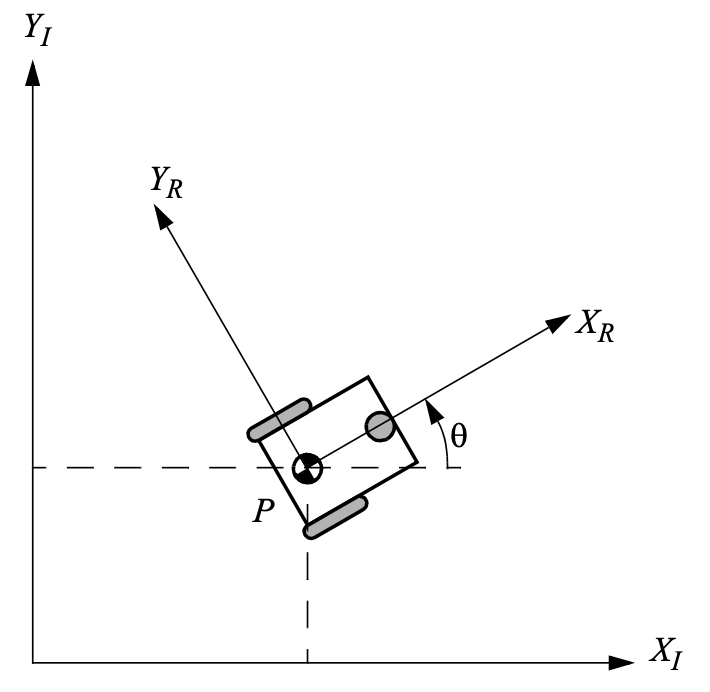
\includegraphics[scale=0.5]{img/3_kinematic_model/reference_frames.png}
    \caption{Le référentiel global et le référentiel local du robot.}
    \label{fig:reference_frames}
\end{figure}

Les axes $\hat{X}_I$ et $\hat{Y}_I$ définissent une base inertielle arbitraire sur le plan en tant que cadre de référence global à partir d'une origine $O:\{ \hat{X}_I, \hat{Y}_I \}$. Pour spécifier la position du robot, nous choisissons un point $P$ sur le châssis du robot, centré entre les deux roues motrices, comme point de référence de sa position. La base $\{\hat{X}_R, \hat{Y}_I \}$ définit deux axes relatifs à $P$ qui constituent donc le cadre de référence local du robot. La position de $P$ dans le cadre de référence global est spécifiée par les coordonnées $x$ et $y$, et la différence angulaire entre les cadres de référence global et local est donnée par $\theta$. Nous pouvons décrire la position du robot comme un vecteur avec ces trois éléments, où l'indice $I$ indique que la base est le cadre de référence global :

\begin{equation}
    \xi = \left [
\begin{array}{l}
     x  \\
     y  \\
     \theta
\end{array}
    \right ]
    \label{eq:position}
\end{equation}

Afin de spécifier la position du robot sur le plan, nous établissons une relation entre le référentiel global du plan et le référentiel local du robot, la \textit{matrice de rotation orthogonale}:
\begin{equation}
    R(\theta) = \left [
    \begin{array}{ccc}
        \cos(\theta) & \sin(\theta) & 0 \\
        -\sin(\theta) & \cos(\theta) & 0 \\
        0 & 0 & 1 \\
    \end{array}
    \right ]
\end{equation}

Cette matrice peut être utilisée pour convertir le mouvement dans le cadre de référence global en mouvement dans le cadre de référence local. Cette opération est dénotée par $\dot{\xi_R} = R(\theta) \cdot \dot{\xi_I}$.

\subsubsection{Forward kinematic models - Modèle cinématique}

Le robot possède deux roues, chacune de diamètre $r$. Étant donné un point $P$ situé entre les deux roues motrices, chaque roue est à une distance $l$ de $P$.

Étant donné $r$, $l$, $\theta$ et la vitesse de rotation de chaque roue, $\dot{\varphi_1}$ et $\dot{\varphi_2}$, un modèle cinématique peut prédire la vitesse globale du robot dans le cadre de référence global: 

\begin{equation}
    \dot{\xi_I} = \left [\begin{array}{c}
        \dot{x} \\
        \dot{y} \\
        \dot{\theta}
        \end{array} \right ]= f \left ( l, r, \theta, \dot{\varphi_1}, \dot{\varphi_2} \right )\\
        == \left [\begin{array}{c}
        \dot{x} \\
        \dot{y} \\
        \dot{\theta}
        \end{array} \right ]
\end{equation}




%\section{Localisation}

La position du robot peut être représenté par l'équation (\ref{eq:position}). À chaque instant, la position peut être estimée à partir d'une position connue en intégrant le mouvement (en additionnant les distances de déplacement incrémentielles).

Pour un système discret avec un intervalle d'échantillonnage fixe $\Delta t$, les distances de déplacement incrémentielles $\left ( \Delta x, \Delta y, \Delta \theta \right )$, c'est-à-dire le chemin parcouru dans le dernier intervalle d'échantillonnage, sont: 
\begin{equation}
    \Delta x = \Delta s \cdot \cos \left ( \theta + \nicefrac{\Delta \theta}{2} \right )
\end{equation}

\begin{equation}
    \Delta y = \Delta s \cdot \sin \left ( \theta + \nicefrac{\Delta \theta}{2} \right )
\end{equation}

\begin{equation}
    \Delta \theta = \frac{\Delta s_r - \Delta s_l}{b}
\end{equation}

\begin{equation}
    \Delta s = \frac{\Delta s_r + \Delta s_l}{2}
\end{equation}

où: 
\begin{itemize}
    \item $\Delta s_r$ et $\Delta s_l$ sont les distances parcourues par la roue droite et la roue gauche, respectivement,
    \item $b$ est distance entre les deux roues du robot.
\end{itemize}


De ce fait, la position mise à jour peut être calculé grâce à:

\begin{equation}
    p' = p + \left [
\begin{array}{l}
     \Delta x  \\
     \Delta y  \\
     \Delta \theta
\end{array}
    \right ] = \left [
\begin{array}{l}
     x  \\
     y  \\
     \theta
\end{array}
    \right ] + \left [
\begin{array}{c}
     \frac{\Delta s_r + \Delta s_l}{2} \cdot \cos \left ( \theta + \frac{\Delta s_r - \Delta s_l}{2\cdot b} \right )  \\
     \frac{\Delta s_r + \Delta s_l}{2} \cdot \sin \left ( \theta + \frac{\Delta s_r - \Delta s_l}{2\cdot b} \right )  \\
     \frac{\Delta s_r - \Delta s_l}{b}
\end{array}
    \right ]
\end{equation}

%%%%%%%%%%%%%%%%%%%%%%%%%%%%%%%%%%%
%%%%%%%%% 3 Février 2022 %%%%%%%%%%
%1. Introduction
%2. Chaîne de communication
%2.1. Implémentation de la chaîne
%2.2. Vérifications - Tests
%3. Formulation de la loi de commande
%3.1. Équations - modèle cinématique (?)
%4. Solution de la loi de commande
%4.1. Matlab
%4.2. Bascule sur C++
%4.3. Vérifications - Tests
%%%%%%%%%%%%%%%%%%%%%%%%%%%%%%%%%%%

\bibliography{bibliography}{}
\bibliographystyle{ieeetr}

% back cover
\imtaMakeCover

\end{document}

